\documentclass{beamer}
\usepackage[utf8]{inputenc}

\usetheme{Madrid}
\usecolortheme{default}
\usepackage{amsmath,amssymb,amsfonts,amsthm}
\usepackage{txfonts}
\usepackage{tkz-euclide}
\usepackage{listings}
\usepackage{adjustbox}
\usepackage{array}
\usepackage{tabularx}
\usepackage{gvv}
\usepackage{lmodern}
\usepackage{circuitikz}
\usepackage{tikz}
\usepackage{graphicx}

\setbeamertemplate{page number in head/foot}[totalframenumber]

\usepackage{tcolorbox}
\tcbuselibrary{minted,breakable,xparse,skins}



\definecolor{bg}{gray}{0.95}
\DeclareTCBListing{mintedbox}{O{}m!O{}}{%
  breakable=true,
  listing engine=minted,
  listing only,
  minted language=#2,
  minted style=default,
  minted options={%
    linenos,
    gobble=0,
    breaklines=true,
    breakafter=,,
    fontsize=\small,
    numbersep=8pt,
    #1},
  boxsep=0pt,
  left skip=0pt,
  right skip=0pt,
  left=25pt,
  right=0pt,
  top=3pt,
  bottom=3pt,
  arc=5pt,
  leftrule=0pt,
  rightrule=0pt,
  bottomrule=2pt,
  toprule=2pt,
  colback=bg,
  colframe=orange!70,
  enhanced,
  overlay={%
    \begin{tcbclipinterior}
    \fill[orange!20!white] (frame.south west) rectangle ([xshift=20pt]frame.north west);
    \end{tcbclipinterior}},
  #3,
}
\lstset{
    language=C,
    basicstyle=\ttfamily\small,
    keywordstyle=\color{blue},
    stringstyle=\color{orange},
    commentstyle=\color{green!60!black},
    numbers=left,
    numberstyle=\tiny\color{gray},
    breaklines=true,
    showstringspaces=false,
}
%------------------------------------------------------------

\title
{2.6.9}
\date{August 26,2025}
\author 
{AI25BTECH11003 - Bhavesh Gaikwad}



\begin{document}


\frame{\titlepage}
\begin{frame}{Question}
\centering
The area of a triangle with vertices A(3,0), B(7,0) and C(8,4) is?
\end{frame}


\begin{frame}[fragile]
    \frametitle{Theoretical Solution}
Given: $A(3,0),\; B(7,0),\; C(8,4).$\\

$
\vec{B}-\vec{A}=\myvec{7-3\\0-0}
=\myvec{4\\0},\qquad
\vec{C}-\vec{A}=\myvec{8-3\\4-0} = \myvec{5\\4}.
$\\

$\norm{\vec{(B-A)} \times \vec{(C-A)}} = \norm{\,\myvec{|\vec{A_{23}} & \vec{B_{23}}| \\ |\vec{A_{31}} & \vec{B_{31}}| \\ |\vec{A_{12}} & \vec{B_{12}}|}\,} = 16 $\\\\


$
\text{Area}=\frac{1}{2}\norm{\vec{(B-A)} \times \vec{(C-A)}} = 8
$

\begin{align}
    \centering
    \boxed{Area \, of \, Triangle \, ABC \,= \,8\,sq.units}
\end{align}

\end{frame}


\begin{frame}[fragile]
    \frametitle{Python + C Code}
    \begin{lstlisting}
#include <stdio.h>
#include <stdlib.h>
#include <math.h>

#ifndef M_PI
#define M_PI 3.14159265358979323846
#endif


#include "matfun.h"
#include "geofun.h"

int main(void) {
    // Allocate 2x1 matrices for points
    double **A = createMat(2,1);
    double **B = createMat(2,1);
    double **C = createMat(2,1);
    \end{lstlisting}
\end{frame}


\begin{frame}[fragile]
    \frametitle{Python + C Code}
    \begin{lstlisting}
        // A(3,0), B(7,0), C(8,4) - correct matrix indexing
    A[0][0] = 3.0; A[1][0] = 0.0;
    B[0][0] = 7.0; B[1][0] = 0.0;
    C[0][0] = 8.0; C[1][0] = 4.0;


    // Vectors B-A and C-A as 2x1 matrices
    double **BA = Matsub(B, A, 2, 1);
    double **CA = Matsub(C, A, 2, 1);

    // Extract components for clarity - correct matrix indexing
    double BAx = BA[0][0], BAy = BA[1][0];
    double CAx = CA[0][0], CAy = CA[1][0];
    \end{lstlisting}
\end{frame}


\begin{frame}[fragile]
    \frametitle{Python + C Code}
    \begin{lstlisting}
    // 2D cross product magnitude |(B-A) x (C-A)| = |BAx*CAy - BAy*CAx|
    double cp = fabs(BAx*CAy - BAy*CAx);
    double area = 0.5 * cp;

    // Save to points.dat
    FILE *fp = fopen("points.dat", "w");
    if (!fp) {
        perror("points.dat");
        // Clean up on error
        freeMat(BA, 2); freeMat(CA, 2);
        freeMat(A, 2); freeMat(B, 2); freeMat(C, 2);
        return 1;
    }
    \end{lstlisting}
\end{frame}



\begin{frame}[fragile]
    \frametitle{Python + C Code}
    \begin{lstlisting}
    fprintf(fp, "# Point_Name X Y\n");
    fprintf(fp, "A %.1f %.1f\n", A[0][0], A[1][0]);
    fprintf(fp, "B %.1f %.1f\n", B[0][0], B[1][0]);
    fprintf(fp, "C %.1f %.1f\n", C[0][0], C[1][0]);
    fclose(fp);
    printf("Wrote points.dat\n");

    // Free memory
    freeMat(BA, 2); freeMat(CA, 2);
    freeMat(A, 2); freeMat(B, 2); freeMat(C, 2);
    
    return 0;
}
\end{lstlisting}
\end{frame}

\begin{frame}[fragile]
    \frametitle{Python + C Code}
    \begin{lstlisting}
import numpy as np
import matplotlib.pyplot as plt
import sys
import os
# Add the triangle folder to the path to import funcs.py
sys.path.append('triangle')
try:
    from funcs import *
except ImportError:
    print("Warning: Could not import from triangle/funcs.py. Using local functions.")
    # Define basic functions if funcs.py is not available
    def tri_sides(A, B, C):
        a = np.linalg.norm(B - C)
        b = np.linalg.norm(C - A)
        c = np.linalg.norm(A - B)
        return c, a, b
    \end{lstlisting}
\end{frame}

\begin{frame}[fragile]
    \frametitle{Python + C Code}
    \begin{lstlisting}
  def read_points_from_file(filename="points.dat"):
    """Read triangle vertices from points.dat file"""
    points = {}
    
    try:
        with open(filename, 'r') as file:
            for line in file:
                # Skip comments and empty lines
                if line.startswith('#') or line.strip() == '':
                    continue
                
                # Parse point data: Point_Name X Y
                parts = line.strip().split()
                if len(parts) == 3:
                    point_name = parts[0]
                    x = float(parts[1])
                    y = float(parts[2])
                    points[point_name] = np.array([x, y])
    \end{lstlisting}
\end{frame}

\begin{frame}[fragile]
    \frametitle{Python + C Code}
    \begin{lstlisting}
      except FileNotFoundError:
        print(f"Error: {filename} not found!")
        return None
    
    return points

def calculate_triangle_area(A, B, C):
    """Calculate triangle area using cross product method"""
    BA = B - A
    CA = C - A
    
    # Cross product magnitude for 2D vectors
    cross_product = abs(BA[0] * CA[1] - BA[1] * CA[0])
    area = 0.5 * cross_product
    
    return area
    \end{lstlisting}
\end{frame}

\begin{frame}[fragile]
    \frametitle{Python + C Code}
    \begin{lstlisting}
  def plot_triangle(A, B, C, area):
    """Plot the triangle with vertices and area annotation"""
    fig, ax = plt.subplots(1, 1, figsize=(10, 8))
    
    # Create triangle vertices array for plotting
    triangle_x = [A[0], B[0], C[0], A[0]]  # Close the triangle
    triangle_y = [A[1], B[1], C[1], A[1]]
    
    # Plot the triangle with orange color
    ax.plot(triangle_x, triangle_y, 'orange', linewidth=2)
    ax.fill(triangle_x, triangle_y, alpha=0.3, color='orange')
    
    # Plot and label vertices
    ax.plot(A[0], A[1], 'ro', markersize=8)
    ax.plot(B[0], B[1], 'go', markersize=8)
    ax.plot(C[0], C[1], 'mo', markersize=8)
    \end{lstlisting}
\end{frame}

\begin{frame}[fragile]
    \frametitle{Python + C Code}
    \begin{lstlisting}
  # Add vertex labels
    ax.annotate(f'A({A[0]:.0f}, {A[1]:.0f})', (A[0], A[1]), 
                xytext=(5, 5), textcoords='offset points', fontsize=12, fontweight='bold')
    ax.annotate(f'B({B[0]:.0f}, {B[1]:.0f})', (B[0], B[1]), 
                xytext=(5, -15), textcoords='offset points', fontsize=12, fontweight='bold')
    ax.annotate(f'C({C[0]:.0f}, {C[1]:.0f})', (C[0], C[1]), 
                xytext=(5, 5), textcoords='offset points', fontsize=12, fontweight='bold')
    
    # Set grid and labels
    ax.grid(True, alpha=0.3)
    ax.set_xlabel('X', fontsize=12)
    ax.set_ylabel('Y', fontsize=12)
    ax.set_title('Triangle ABC', fontsize=14, fontweight='bold')
    \end{lstlisting}
\end{frame}

\begin{frame}[fragile]
    \frametitle{Python + C Code}
    \begin{lstlisting}
    # Set axis limits with some padding
    x_min, x_max = min(A[0], B[0], C[0]) - 1, max(A[0], B[0], C[0]) + 1
    y_min, y_max = min(A[1], B[1], C[1]) - 1, max(A[1], B[1], C[1]) + 1
    ax.set_xlim(x_min, x_max)
    ax.set_ylim(y_min, y_max)
    
    # Equal aspect ratio
    ax.set_aspect('equal', adjustable='box')
    
    # Save the plot
    plt.tight_layout()
    plt.savefig('triangle_plot.png', dpi=300, bbox_inches='tight')
    plt.show()
    \end{lstlisting}
\end{frame}

\begin{frame}[fragile]
    \frametitle{Python + C Code}
    \begin{lstlisting}
  def main():
    print("Triangle Area Calculator and Plotter")
    print("=" * 40)
    
    # Read points from file
    points = read_points_from_file("points.dat")
    
    if points is None:
        print("Failed to read points from file.")
        return
    
    # Extract vertices
    try:
        A = points['A']
        B = points['B']
        C = points['C']
    \end{lstlisting}
\end{frame}

\begin{frame}[fragile]
    \frametitle{Python + C Code}
    \begin{lstlisting}   
        print(f"Points read from file:")
        print(f"A = ({A[0]:.1f}, {A[1]:.1f})")
        print(f"B = ({B[0]:.1f}, {B[1]:.1f})")
        print(f"C = ({C[0]:.1f}, {C[1]:.1f})")
        print()
        
    except KeyError as e:
        print(f"Error: Missing point {e} in points.dat")
        return
    
    # Calculate area using the cross product method
    area = calculate_triangle_area(A, B, C)
    
    # Display calculation steps (similar to the image)
    BA = B - A
    CA = C - A
    \end{lstlisting}
\end{frame}

\begin{frame}[fragile]
    \frametitle{Python + C Code}
    \begin{lstlisting}
      
    print("Solution:")
    print(f"Given: A({A[0]:.0f},{A[1]:.0f}), B({B[0]:.0f},{B[1]:.0f}), C({C[0]:.0f},{C[1]:.0f})")
    print()
    print(f"B - A = ({BA[0]:.0f}, {BA[1]:.0f})")
    print(f"C - A = ({CA[0]:.0f}, {CA[1]:.0f})")
    print()
    
    cross_product = abs(BA[0] * CA[1] - BA[1] * CA[0])
    print(f"|(B - A) * (C - A)| = |{BA[0]:.0f} * {CA[1]:.0f} - {BA[1]:.0f} * {CA[0]:.0f}| = {cross_product:.0f}")
    print()
    print(f"Area = (1/2) * |(B - A) * (C - A)| = (1/2) * {cross_product:.0f} = {area:.0f}")
    print()
    print(f"Area of Triangle ABC = {area:.2f} sq.units")
    print()
    \end{lstlisting}
\end{frame}

\begin{frame}[fragile]
    \frametitle{Python + C Code}
    \begin{lstlisting}
      # Try to calculate side lengths if funcs.py is available
    try:
        sides = tri_sides(A, B, C)
        print(f"Triangle side lengths:")
        print(f"AB (c) = {sides[0]:.2f}")
        print(f"BC (a) = {sides[1]:.2f}")
        print(f"CA (b) = {sides[2]:.2f}")
        print()
    except NameError:
        print("tri_sides function not available")
    
    # Plot the triangle
    plot_triangle(A, B, C, area)
    
    print("Triangle plot saved as 'triangle_plot.png'")

if __name__ == "__main__":
    main() 
    \end{lstlisting}
\end{frame}


\begin{frame}{Graph}
   \centering
    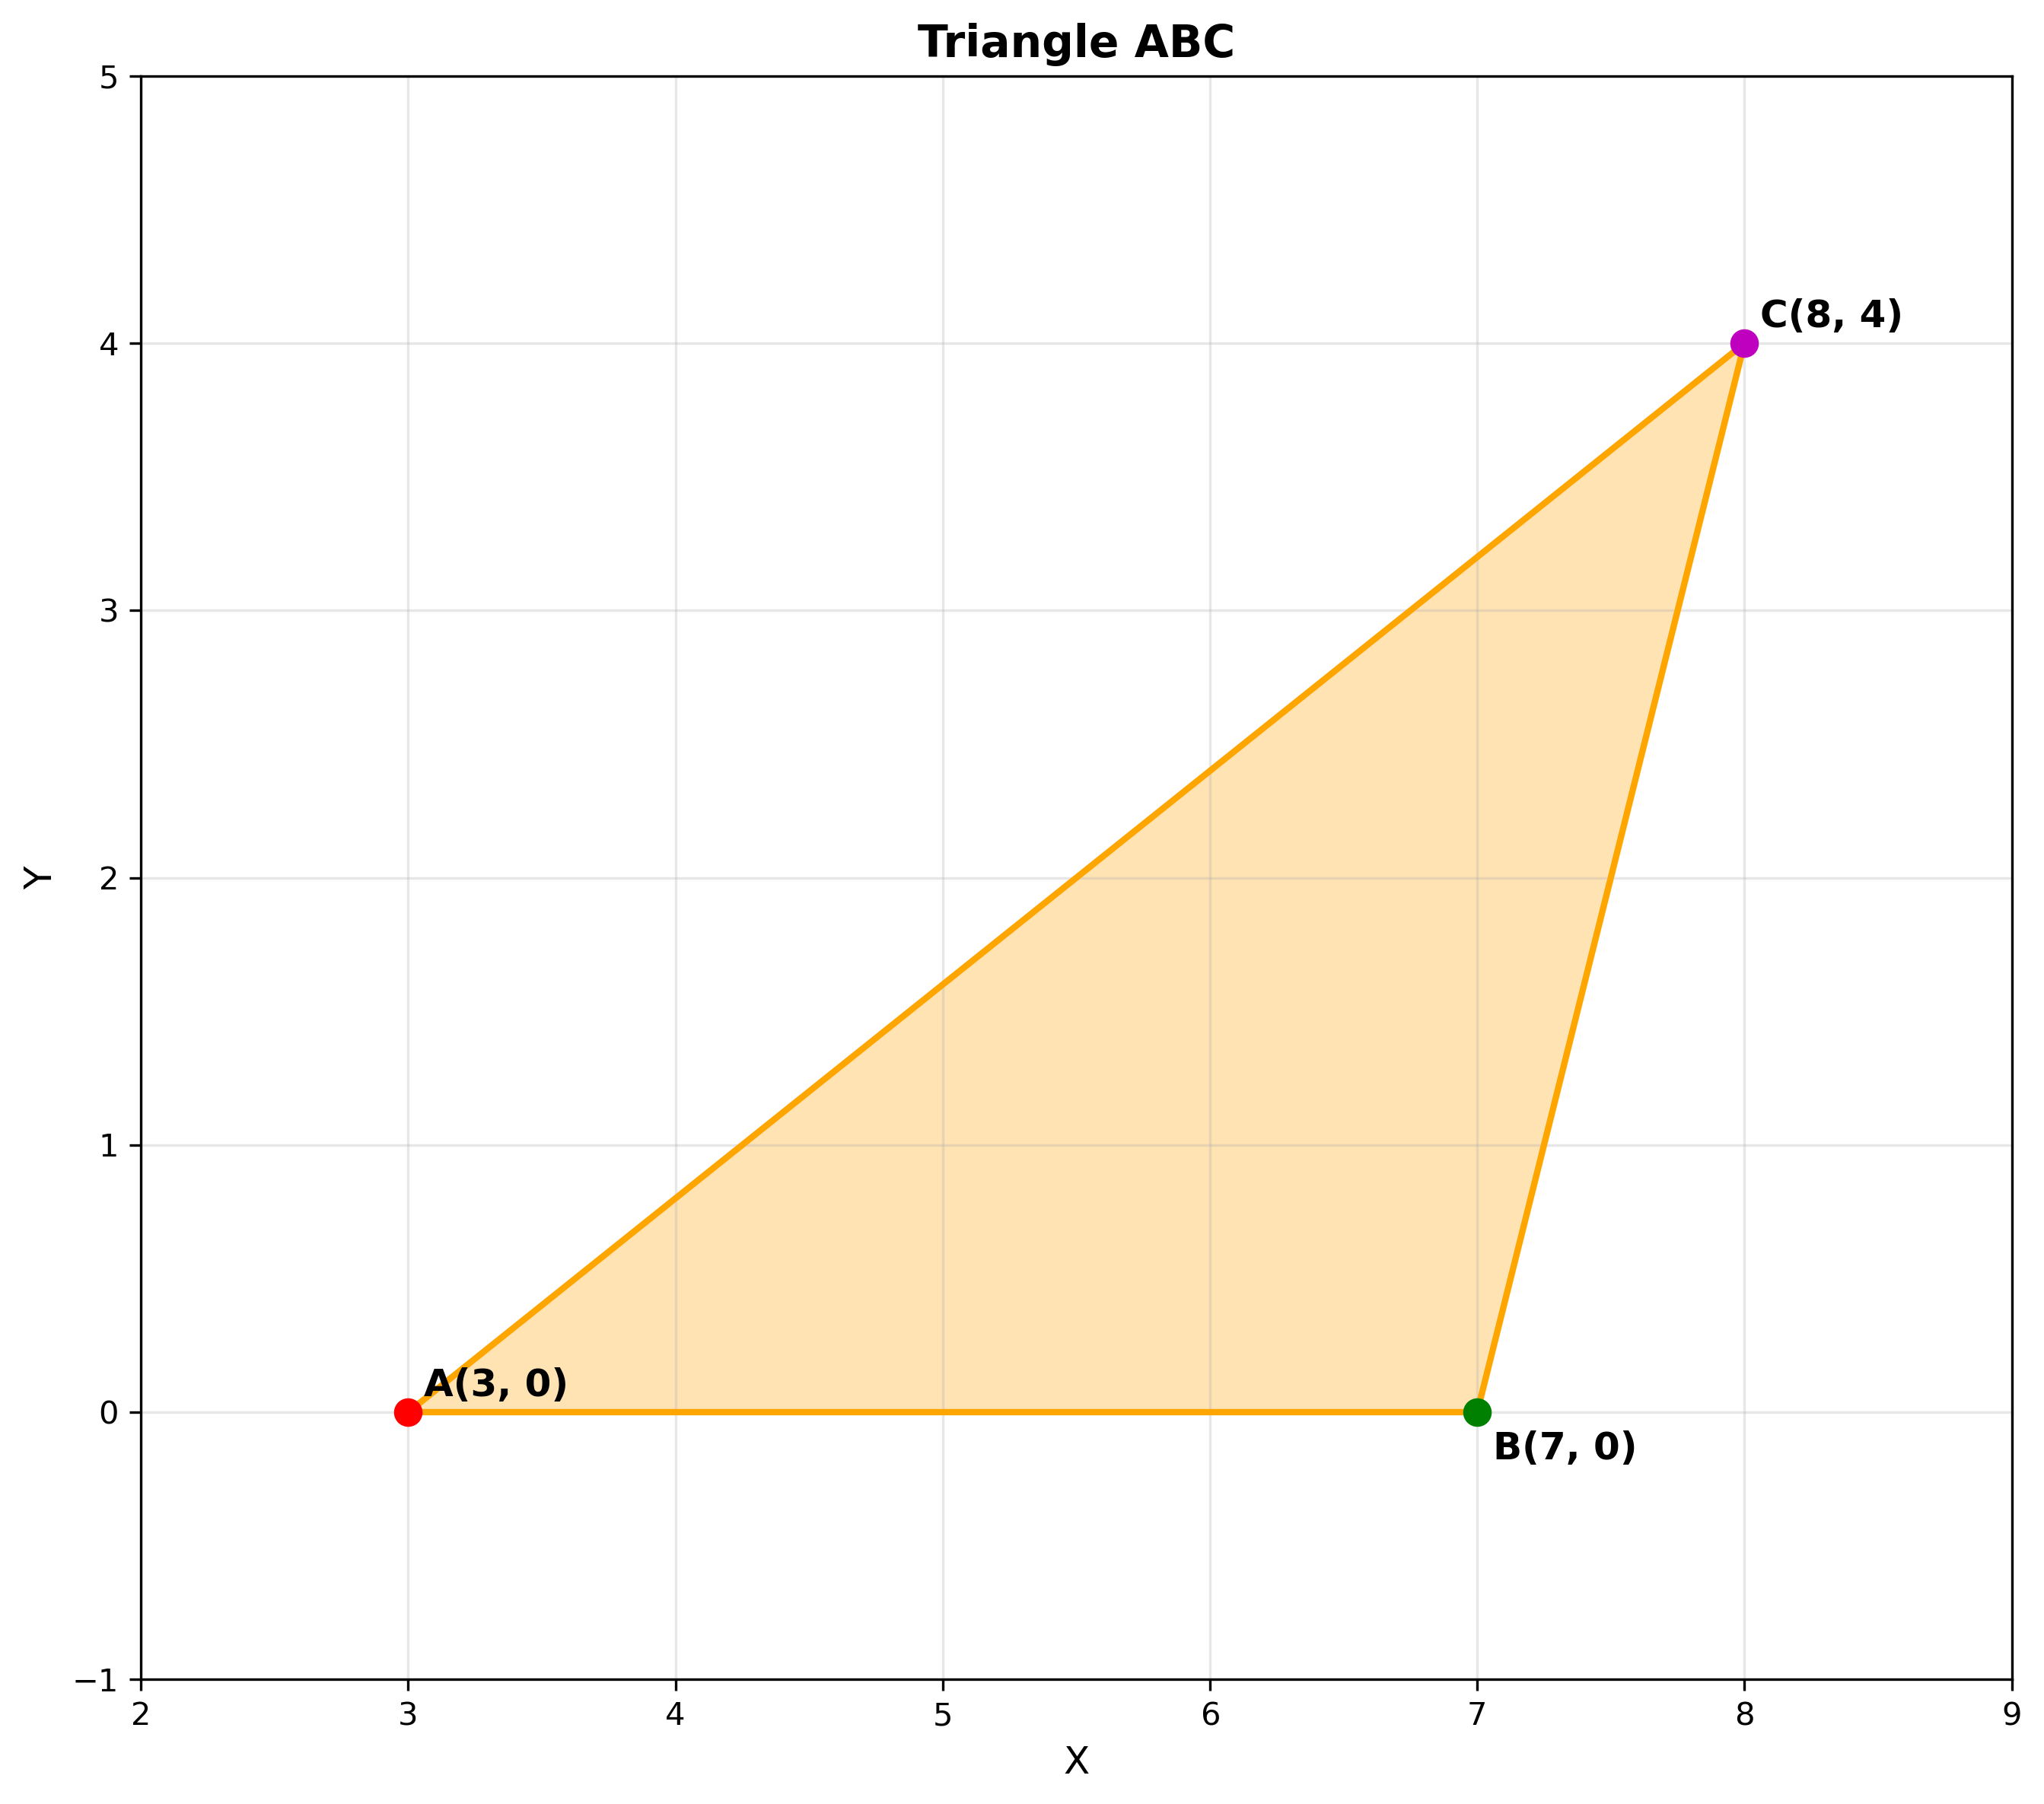
\includegraphics[width=\columnwidth, height=0.8\textheight, keepaspectratio]{figs/fig1.png}
    \label{fig:Beamer/figs/fig1.png}
\end{frame}


\end{document}